\documentclass{article}
%\usepackage{standalone}
\usepackage{fancyhdr}


\usepackage{import}
\usepackage{caption}
\usepackage{amsfonts, amsmath, amsthm}
\usepackage{makecell}
\usepackage{lastpage}
\usepackage{moresize}



\hyphenpenalty=10000


\usepackage[utf8x]{inputenc}
\usepackage[T1]{fontenc}
\usepackage[english]{babel}
\usepackage{graphicx}
%\usepackage[languagenames,fixlanguage,english]{babelbib}
\usepackage[pdftex]{hyperref}
%\usepackage{txfonts}
\usepackage{subcaption}
\usepackage[a4paper,top=3cm,bottom=2cm,left=3cm,right=3cm,marginparwidth=1.75cm]{geometry}
\usepackage{algorithm2e}
\usepackage{pdflscape}

\usepackage[e]{Template/gameshf}






\usepackage{tikz}
\usepackage{pgfplots}
\usepackage{circuitikz}
\usepackage{tabularx}
\usepackage{rotating}
\usepackage{caption} 
\captionsetup[table]{skip=10pt}

\usetikzlibrary{calc,positioning,shapes,decorations.pathreplacing}

\tikzset{
	short/.style={draw,rectangle,text height=3pt,text depth=13pt,
		text width=7pt,align=center,fill=gray!30},
	long/.style={short,text width=1.5cm},
	verylong/.style={short,text width=4.5cm}
}


%% User defined
\newcommand{\N}{\mathbb{N}}
\newcommand{\Z}{\mathbb{Z}}
\newcommand{\Q}{\mathbb{Q}}
\newcommand{\R}{\mathbb{R}}
\newcommand{\C}{\mathbb{C}}
\newcommand{\funcA}{\mathfrak{a}}
\newcommand{\funcB}{\mathfrak{b}}
\newcommand{\funcC}{\mathcal{C}}
\newcommand{\funcU}{\mathcal{U}}
\newcommand{\funcV}{\mathcal{V}}
\newcommand{\funcW}{\mathcal{W}}
\newcommand{\simgrad}{\sym\nabla}
\newcommand{\heps}{{h,\varepsilon}}
\newcommand{\epsh}{{\varepsilon(h)}}
\newcommand{\eps}{{\varepsilon}}
\newcommand{\twoscale}{{\,\overset{2}{\rightharpoonup}\,}}
\newcommand{\drtwoscale}{{\,\overset{dr-2}{\rightharpoonup}\,}}
\DeclareMathOperator{\sym}{sym}
\DeclareMathOperator{\dvg}{div}

%\newtheorem{exmp}{Example}[section]
%\newtheorem{note}{Note}
%\newtheorem{theorem}{Theorem}[section]
%\newtheorem{proposition}[theorem]{Proposition}
%\newtheorem{corollary}{Corollary}
%\newtheorem{definition}[theorem]{Definition}
%\newtheorem{lemma}{Lemma}[theorem]

\headheight 40pt              %% put this outside
\headsep 10pt                 %% put this outside


\graphicspath{{./Images/Crane/}{./Images/Electronics/}}

% Source: 
%https://tex.stackexchange.com/questions/117990/unicode-math-breaks-declaremathoperator
\AtBeginDocument{
	\let\div\relax
	\DeclareMathOperator{\div}{div}
}

\usepackage{enumitem}
\setlist[description]{style=unboxed}

%opening
\title{STEM games 2019}
\author{Mentori}

\title{STEM Games Engineering Arena}
\date{}

\begin{document}
	%\maketitle
	
	\thispagestyle{empty}
	\newpage
	\thispagestyle{empty}
	\vspace*{0cm}
	\begin{center}
		
		\textbf{\Huge{STEM Games 2019}}\\
		\vspace*{2.4cm}
		
\includegraphics[width=0.4\textwidth]{logos/engineering} \\
		\vspace*{2.4cm}
		% TODO naslov
		\huge{UNDERWATER HABITATS}
		
		\medskip
		
		\normalsize{a problem by}
		
		\medskip
		
		Dominik Barbarić \\
		Karla Draženović \\
		Nenad Ferdelji \\
		Ante Orešković \\
		Ivan Pavić \\
		Vedra Slapničar \\
		Danijel Zadravec \\
		Marko Švec 
		
		\vspace{6cm}
		
		
		% TODO Neki mini tekst?
		\normalsize{}
	\end{center}

	\newpage
	\section{Arena introduction}
	
	Firstly, i want to welcome all the contestants that will be competing in 
	2019 STEM Games engineering arena!
	
	This year's task focuses on the underwater habitats and logistical problems 
	around them.
	Underwater habitats are permanent and semi-permanent habitats located at 
	the sea beds.
	They provide all facilities required for the human survival
	
	\newpage
	\section{Introduction}
	
	\noindent 
	\textbf{Friendly advice}: Read everything before solving the task. Task grading is automatic. Submission form for every task is described in task's readme file.
	
	\section{Tasks} \label{sec:tasks}
	
	The system for which you have to design a controller is the crane shown in the Figure \ref{fig:isometry}. The crane consists of a base, two booms(in some crane configurations \textit{Boom 1} is also called \textit{Mast}), two telescopic beams, three hydraulic cylinders, two electric motors and pulley with belt system. The purpose of the crane is to load the submarine with goods and equipment which is to be transported to underwater habitats.Masses of each part of the crane are listed in Table \ref{tab:crane_tab}.\textbf{ For the sake of simplicity and overall system dynamics, load has the mass $m_{load} = 800.59 kg$}.
	
	\begin{figure}[h!]
		\centering
		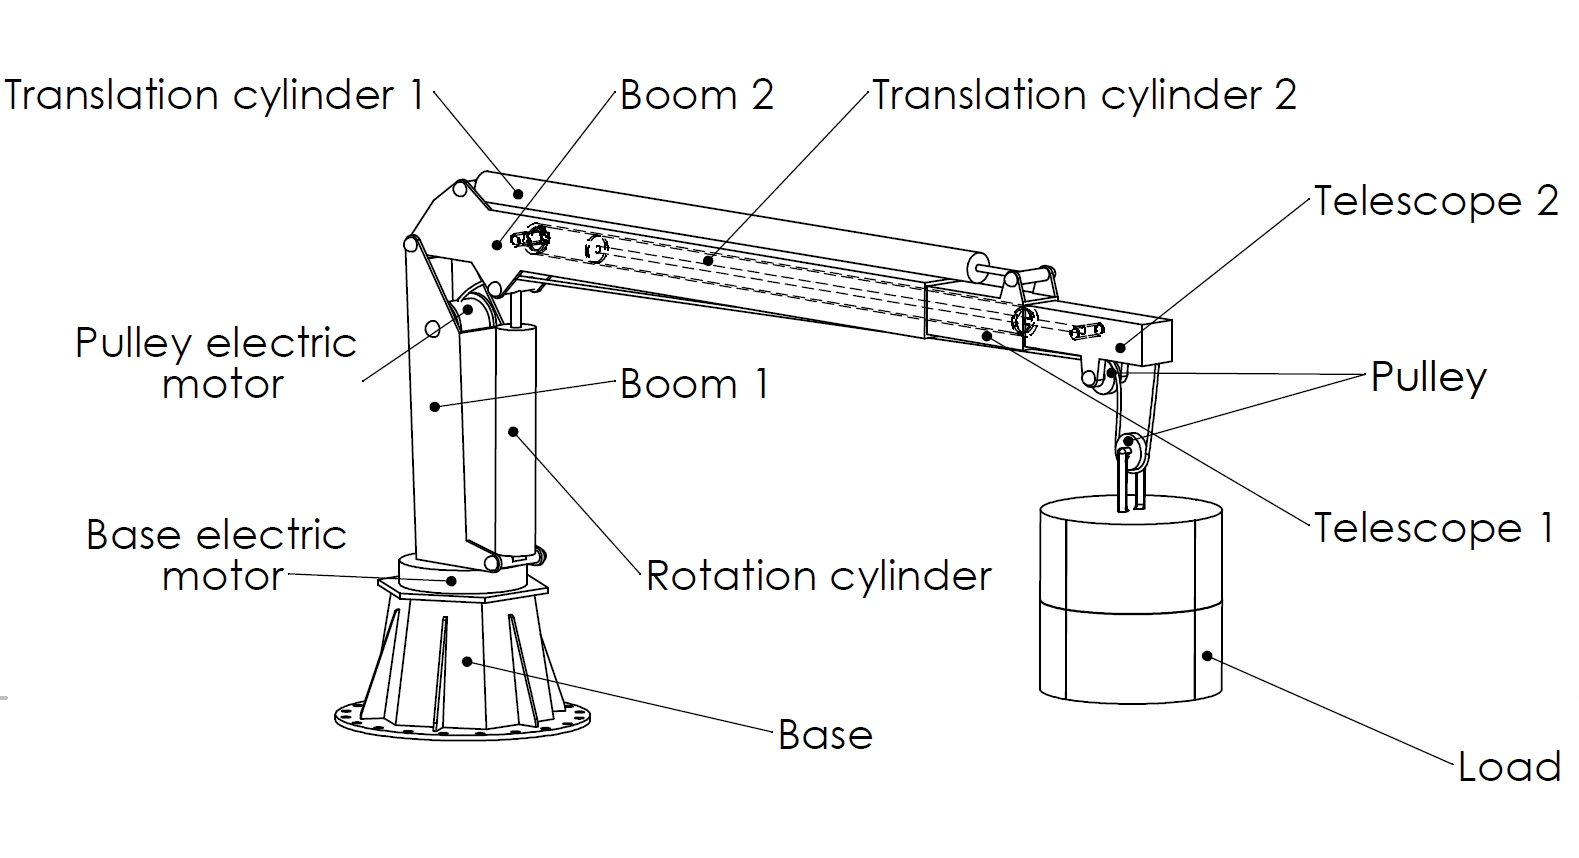
\includegraphics[width=\textwidth]{kran_teret_izometrija.jpg}
		\caption{Crane configuration, isometry.}
		\label{fig:isometry}
	\end{figure}
	
	\begin{center}
		\captionof{table}{Crane mass}\label{tab:crane_tab}
		\begin{tabular}{||c|| c || c|| c ||}
			\hline
			Part & Mass$[kg]$ & Part & Mass$[kg]$ \\
			\hline\hline
			Base + Base electric motor & 3794.43 & Rotation cylinder & 105.30\\ 
			\hline
			Boom 1 & 536.36 & Translation cylinder 1 & 199.42\\
			\hline
			Boom 2 & 807.88 & Translation cylinder 2 & 198.24\\
			\hline
			Telescope 1 & 664.18 & Pulley & 12.25\\
			\hline
			Telescope 2 & 611.33 & Pulley electric motor & 47.23\\
			\hline
		\end{tabular}
	\end{center}
	
	\subsection{Hydraulics system}
	
	Part of the crane is actuated using hydraulic system. The system, as we designed it, is shown in Figure \ref{fig:hydraulic} and we are aware it has some flaws. Your first task is to think about how you could redesign the system and improve its performance. Concentrate on what you can conclude with what we have given you, i.e. we ask you to propose a redesign of the schematics. You might want to postpone this task until you are done with other tasks and have a better understanding of the system you are working with.
	
	\begin{figure}[h!]
		\centering
		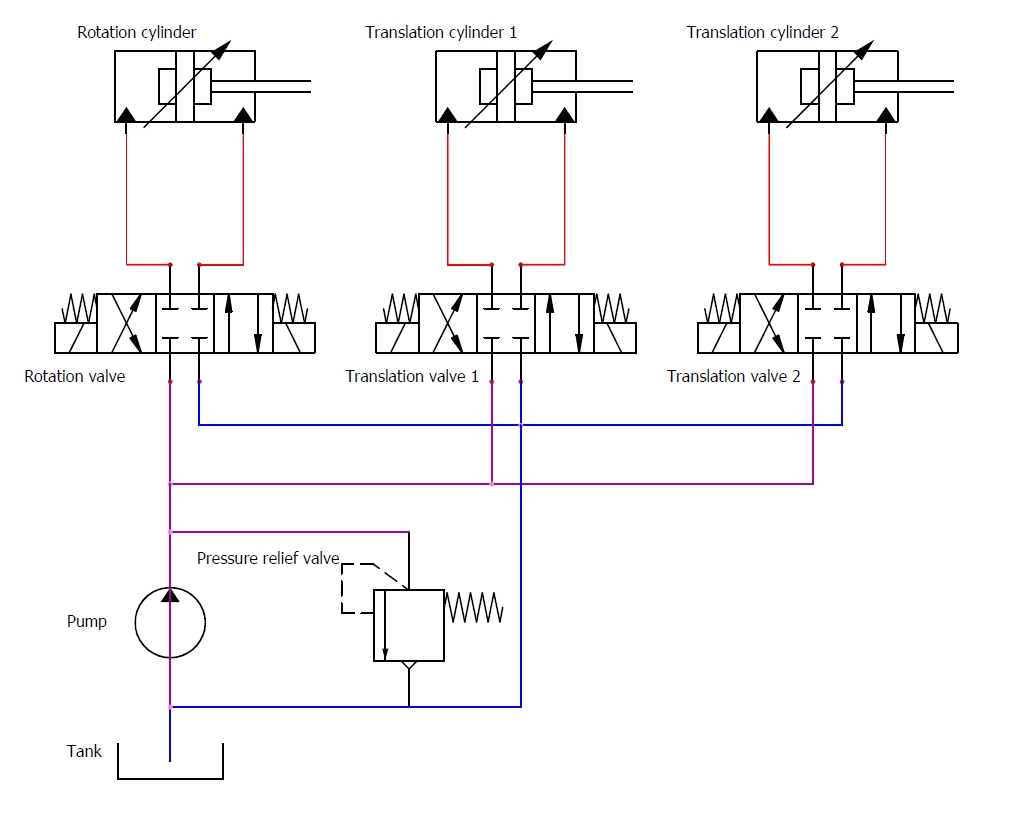
\includegraphics[width=0.75\textwidth]{hidraulika_shema.jpg}
		\caption{Hydraulic system schematics.}
		\label{fig:hydraulic}
	\end{figure}
	
	\subsection{Kinematics}

	Kinematics model of the crane is important to ensure that the cargo is 
	precisely placed into the submarine which delivers it to underwater 
	habitats.
	
	Crane configuration and dimensions are shown in Figure \ref{fig:crane_side}, Figure \ref{fig:crane_top} and Figure \ref{fig:crane_back}. Figure \ref{fig:cylinder_conf} shows cylinder configuration with corresponding dimensions given in Table \ref{tab:cylinder_tab}. Load is shown in Figure \ref{fig:load}.
	
	\begin{figure}[h!]
		\centering
		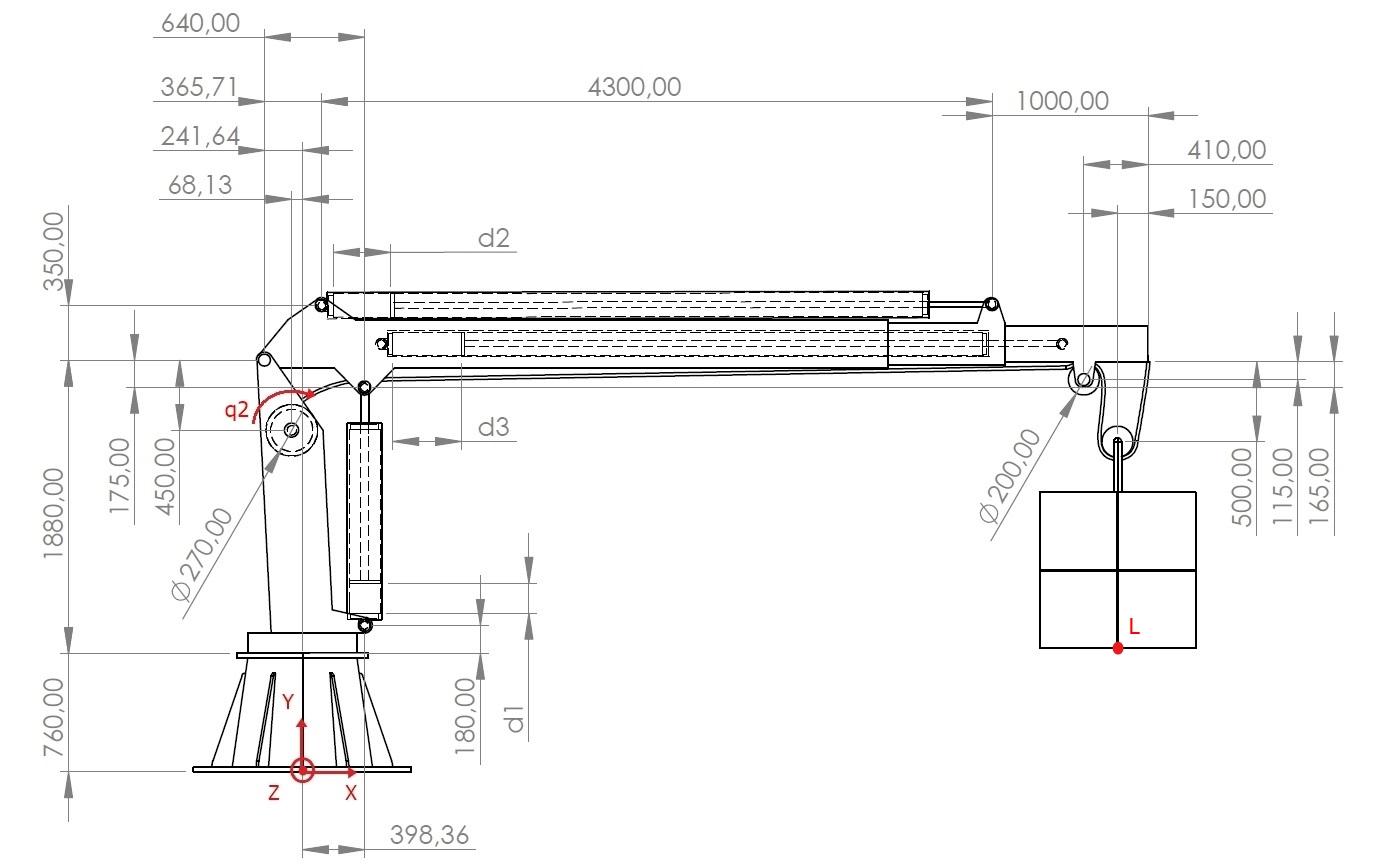
\includegraphics[width=\textwidth]{kran_bokocrt.jpg}
		\caption{Crane configuration, side view.}
		\label{fig:crane_side}
	\end{figure}
	
	\begin{figure}[h!]
		\centering
		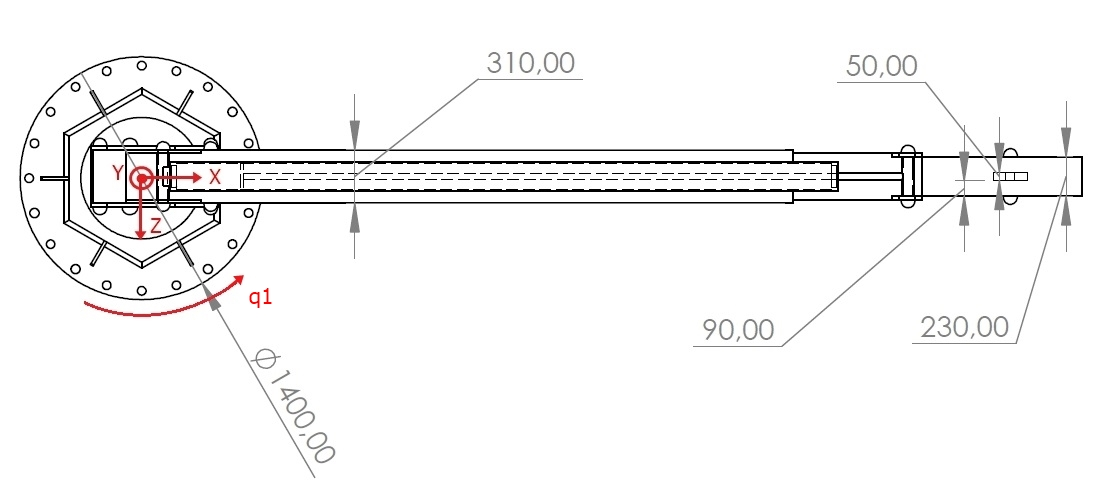
\includegraphics[width=\textwidth]{kran_tlocrt.jpg}
		\caption{Crane configuration, top view.}
		\label{fig:crane_top}
	\end{figure}
	
	\begin{figure}[h!]
		\centering
		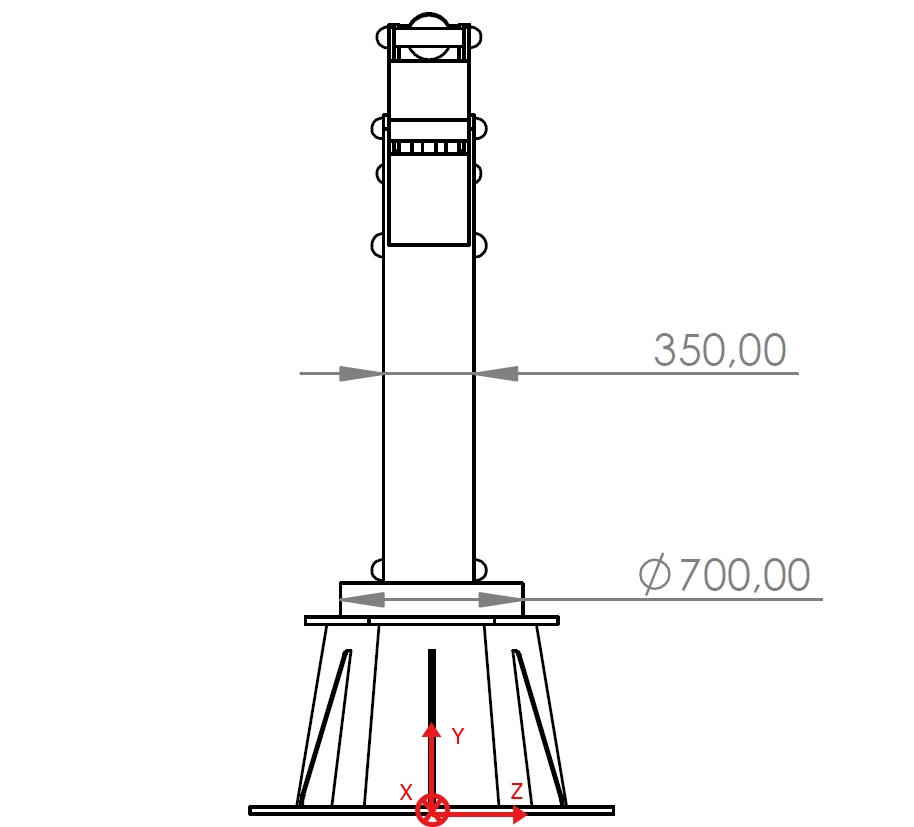
\includegraphics[width=0.65\textwidth]{kran_nacrt.jpg}
		\caption{Crane configuration, back view.}
		\label{fig:crane_back}
	\end{figure}
	
	\noindent
	\textbf{Crane configuration has been sketched for $q_1 = 0 ^\circ$, $d_1 = 
	194mm$, $d_2 = 369mm$, $d_3 = 437.22mm$ and $q_2 = 0 ^\circ$. Base 
	coordinate system is defined by red coordinate axes while red dot $L$ 
	represents bottom of the load.} Limits of motor angles and cylinder offsets 
	are given in Table \ref{tab:limits}.
	
	\begin{center}
		\captionof{table}{Actuator position limits}\label{tab:limits}
		\begin{tabular}{|| c || c c c c c ||}
			\hline
			Variable & $q_1[^{\circ}]$ & $d_1$[m] & $d_2$[m] & $d_3$[m] &  
			$q_2[^{\circ}]$\\
			\hline\hline
			Minimum value & $\times$ & 0 & 0 & 0 & 0 \\ 
			\hline
			Maximum value & $\times$ & 0.8 & 3.5 & 3.5 & 20000 \\ 
			\hline
		\end{tabular}
	\end{center}
	
	\begin{figure}
		\centering
		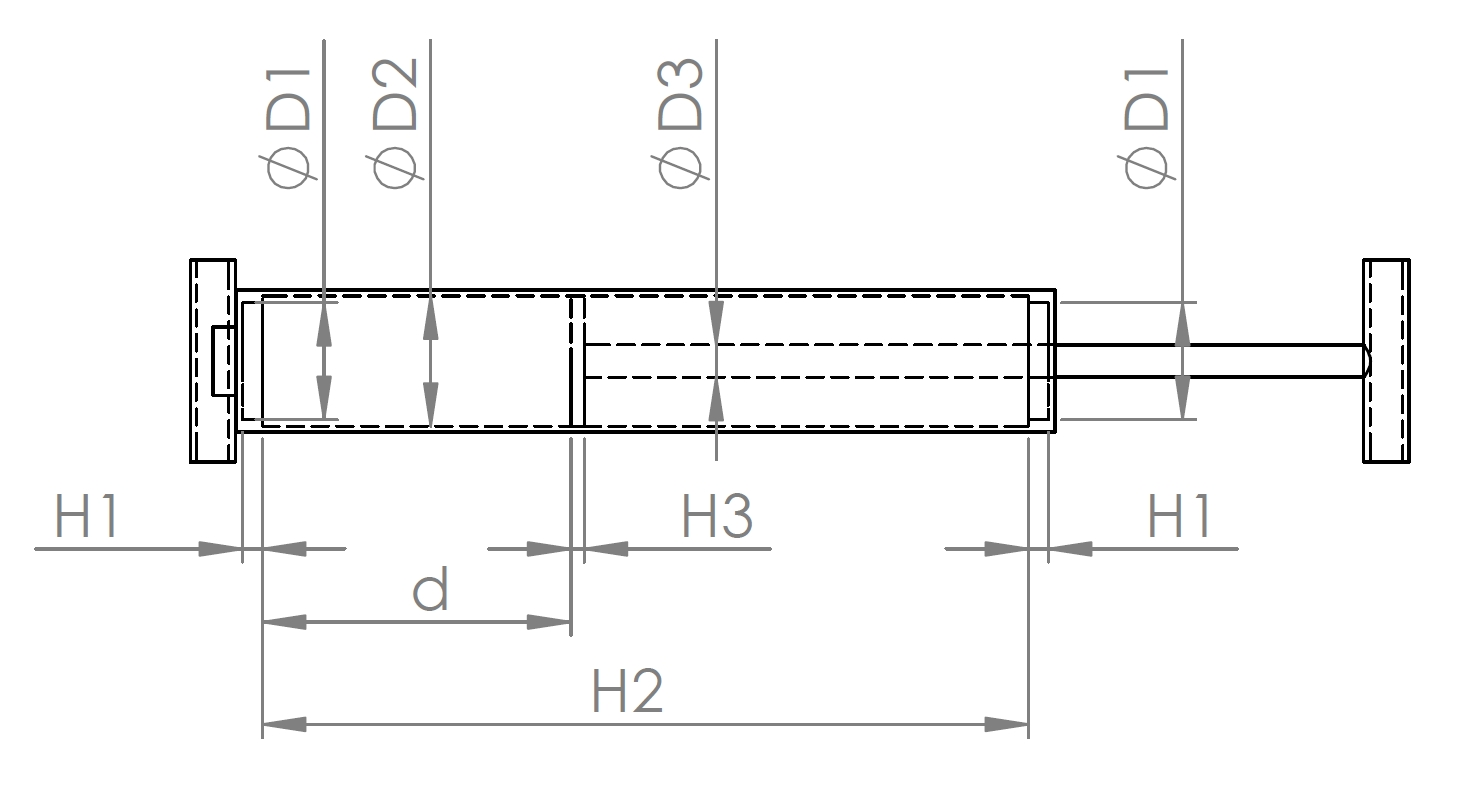
\includegraphics[width=0.75\textwidth]{cilindar_shema.jpg}
		\caption{Cylinder configuration with dimensions.}
		\label{fig:cylinder_conf}
	\end{figure}
	
	\begin{center}
		\captionof{table}{Cylinder dimensions}\label{tab:cylinder_tab}
		\begin{tabular}{||c|| c c c || c c c ||}
			\hline
			Cylinder & D1[mm] & D2[mm] &  D3[mm] & H1[mm] & H2[mm] & H3[mm] \\
			\hline\hline
			Rotation & 180 & 200 & 50 & 30 & 820 & 20\\ 
			\hline
			Translation & 80 & 100 & 37.5 & 30 & 3520 & 20 \\
			\hline
		\end{tabular}
	\end{center}
	
	\begin{figure}[h!]
		\centering
		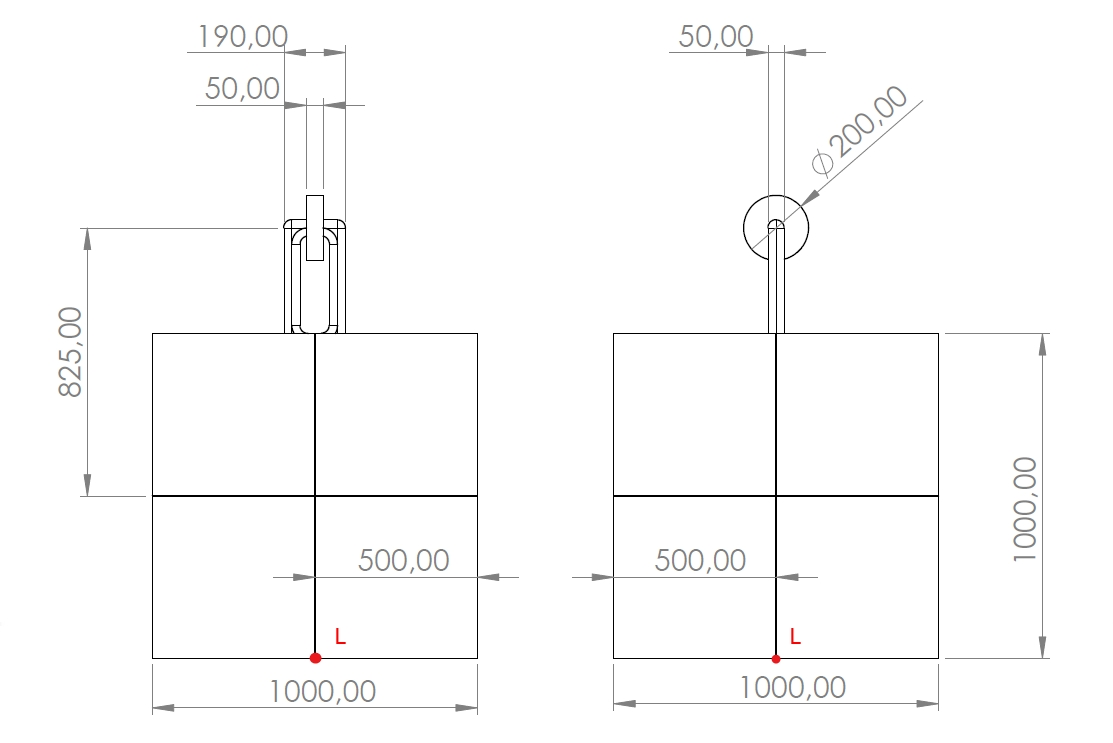
\includegraphics[width=0.8\textwidth]{teret.jpg}
		\caption{Load}
		\label{fig:load}
	\end{figure}
	
	\subsubsection{Direct}
	
	To be able to design a controller, first you have to understand  kinematics of the crane. Your task is to find the position of the load $L(x_L,y_L,z_L)$ for every combination of electric motor angles and cylinder offsets given in Table \ref{tab:direct}. Be careful calculating the result because \textbf{maximum offset} from correct solution we will tolerate is $\pm 0.25$ m.
	\noindent NOTE: Pulley is trickier than it looks.
	
	
	\begin{center}
		\captionof{table}{Direct kinematics configurations}\label{tab:direct}
		\begin{tabular}{|| c || c c c c c ||}
			\hline
			Configuration & $q_1[^{\circ}]$ & $d_1$[m] & $d_2$[m] & $d_3$[m] &  
			$q_2[^{\circ}]$\\
			\hline\hline
			1. & 0 & 0.194 & 1 & 1 & 1500 \\ 
			\hline
			2. & 45 & 0.4 & 0 & 2 & 3600 \\
			\hline
			3. & 90 & 0.7 & 3.5  & 3.5 & 5000 \\
			\hline
		\end{tabular}
	\end{center}
	
	\noindent
	Information on how to submit your solution will be given to you in the \textit{readme} file in task folder. If you have any questions regarding submission of the task, ask your mentors.
	
	\subsubsection{Inverse}
	
	Next step is to be able to determine kinematic configuration in opposite direction. Based on load positions specified in Table \ref{tab:inverse}, determine the corresponding angles and offsets $(q_1, d_1, d_2, d_3, q_2)$ for every given configuration. It is often the case that inverse kinematics has multiple valid solutions, so any valid solution you give will be graded as successful. We will set the crane in configuration position you give us and check if it is inside the maximum offset range of $\pm 0.25$ m from reference point given in Table \ref{tab:inverse}.
	
	\begin{center}
		\label{tab:inverse}
		\captionof{table}{Inverse kinematics configurations}\label{tab:inverse}
		\begin{tabular}{|| c || c c c ||}
			\hline
			Configuration & $x_L$[m] & $y_L$[m] & $z_L$[m] \\
			\hline\hline
			1. & 8.0 & -5.0 & 0.0\\ 
			\hline
			2. & -7.5 & -5.0 & 7.5 \\
			\hline
			3. & 0.0 & 0.5 & 2.5 \\
			\hline
		\end{tabular}
	\end{center}
	
	\noindent
	Information on how to submit your solution will be given to you in the \textit{readme} file in task folder. If you have any questions regarding submission of the task, ask your mentors.
	
	\subsection{Model identification}
	
	Now when you understand kinematics of the crane, it would be useful to know its dynamic model.
	
	As mentioned before, the crane has 5 actuators. There is a DC motor which is turning the whole crane, one hydraulic actuator performing rotation of booms and telescopes (lifting), two hydraulic actuators used for extension of telescopes and finally a DC motor running belt and pulley system. To successfully drive the crane, you have to determine how it reacts to given inputs. In real systems, you often don't know how system will respond to your inputs, mostly because the model of the system is unknown. In many cases, there are some unknown parameters, order of model is unknown or maybe some parameters are not correct due to the age of system you are controlling, for example, old batteries, old motors, etc.
	
	For this task you will do exactly that! Some of the parameters of the system are unknown and there is no way to measure them so you have to identify models for all crane actuators.
	
	Crane is set to default start position ($q_1 = 0; \ d_1 = 0.194; \  d_2 = 0; \  d_3 = 0; \  q_2 = 0$) and it is ready for driving. Given the known parameters of actuators (Table ), your job is to determine how the actuator will respond. We give you the opportunity to test whatever input signals you want.
	Inputs for DC motors are in Volts [V] and for hydraulic actuators are valve opening in Meters[m]. Input signal limits are given in Table \ref{tab:input_limits}.  In task's \textit{readme} file you can find a way how to test your input signals and submit your results.
	
	\begin{center}
		\label{tab:inverse}
		\captionof{table}{Electric motor parameters}\label{tab:el_params}
		\begin{tabular}{|| c || c c c c c||}
			\hline
			Parameter & R[$\Omega$] & $L$[mH] & $k$[Vs/rad] & $J_{rot}$[kgm$^2$] & 
			$n$\\
			\hline\hline
			Base electric motor & 2.3 & 20 & 1.3 & 0.2 & 200\\ 
			\hline
			Pulley electric motor & 1.7 & 12 & 1.6 & 0.1 & 20\\
			\hline
		\end{tabular}
	\end{center}
	
	\begin{center}
		
		\captionof{table}{Actuator input signal limits}\label{tab:input_limits}
		\begin{tabular}{|| c || c c c c c ||}
			\hline
			Actuator & \makecell{Base electric \\ motor [V]} & \makecell{Rotation \\ cylinder \\ valve[m]} & \makecell{Translation \\ cylinder 1 \\ valve[m]} & \makecell{Translation \\ cylinder 2 \\ valve[m]} &  \makecell{Pulley electric \\ motor [V]}\\
			\hline\hline
			\makecell{Minimum \\ value} & -120 & -0.005 & -0.005 & -0.005 & -180 \\ 
			\hline
			\makecell{Maximum\\ value} & 120 & 0.005 & 0.005 & 0.005 & 180 \\ 
			\hline
		\end{tabular}
	\end{center}
	
	We will test your solution with randomly generated test signals. To prevent you from sending us your test signal as an input for identification, every time you send signal for identification we will create new test signal and \textbf{erase all your previous results}. That means that after you decide that your test identification is good enough for you, you should not send another identification signal.
	As said before, test signals are generated randomly. In total, you will have 5 test cases.  Each test case will start in default start position . 
	Identification signal for every actuator is \textbf{step} function  (Heaviside function) with random step time in interval [0, $T_{sim}$] and with random value amplitude. Example of one test signal can be found in the task folder.
	
	\subsection{Crane driving}
	
	After creating both kinematic and dynamic models of the system, your task is to make it serve its purpose. Crane has to carry a specific cargo from the dock to the submarine cargo space. Desired positions are given in Table \ref{tab:inverse} and you have already calculated inverse dynamics for these coordinates. Crane has to place the load in these points in the order given in Table \ref{tab:trajectory}.
	
	\begin{center}
		\captionof{table}{Desired crane positions}\label{tab:trajectory}
		\begin{tabular}{|| c c c c c ||}
			\hline
			$P_1$ & $P_2$ & $P_3$ & $P_4$ & $P_5$\\
			\hline\hline
			3 & 1 & 3 & 2 & 3  \\ 
			\hline
		\end{tabular}
	\end{center}
	
	\noindent
	At each stop, the load has to stay steady for at least $t_{steady} = 5s$ before proceeding to the next one. "Stay steady" in this context means that the bottom point $L(x_L,y_L,z_L)$ of the load has to stay in the norm ball of $R = 0.25$ m around the reference point. Test is finished after the load has been in all requested positions or when the maximum simulation time $T_{sim} = 250s$ has passed. This is measured using test time $T_{test}$. Final performance cost $J_{total}$ is calculated using the following expression:
	
	\begin{equation} \label{eq:total_cost}
	J_{total} = \frac{5}{24}\sum_{i=1}^{5} D_i + \frac{75}{2} T_{total},
	\end{equation}
	
	\begin{equation} \label{eq:distance_cost}
	D_i = \left\{
	\begin{array}{ll}
	\sum_{t=T_{i-1}}^{T_{i}} ||L(t) - P_i||, &  P_i \textrm{ reached}, \\
	& \\
	10000, &  P_i \textrm{ not reached},\\
	\end{array} 
	\right.
	\end{equation}
	
	\noindent
	where $T_i$ is the time in which $t_{steady}$ has been reached in position $P_i$ and $T_0 = 0s$.
	
	\vspace{10pt}
	\noindent
	Your task is to design five controllers, one for every actuator. 
	Discretization time for every controller is $T_s = 50ms$. Information on 
	how to submit your solution will be given to you in the \textit{readme} 
	file in task folder. If you have any questions regarding submission of the 
	task, ask your mentors.
	
\newpage
\section{DC voltage power supply}

\subsection{Introduction}

For fully functional operation, the crane is equipped with 
lot of computer based subsystems and electronic devices which operate on DC 
voltage. To ensure their proper operation the, DC voltage has to be stable and 
without noise. To ensure stable DC voltage, device on Fig. 
\ref{fig:schematic}. is used. Device is composed of several parts as it is 
shown on the figure. Due to extreme conditions in the system, regulators often 
fail and components have to be repaired or replaced with proper spare part.

In this task, your job is to:
\begin{itemize}
	\item find the parts which ensure proper operation of regulator, 
	\item ensure that the output voltage ripple is within the boundaries with 
	proper choice of parts for the low pass filter,
	\item find the probability of future malfunction in standby redundant 
	system.
\end{itemize}

\textbf{Device specifications.} Device specifications are provided with 
the following table. In the first and the second task you have to choose device 
components. You have to ensure that your choice guarantees that the 
device operating parameters are within the requirements specified in the 
table \ref{tab:spec}.

\begin{table}[h!]
	\hyphenpenalty 10000
	\caption{Device specifications}
	\label{tab:spec}
	\begin{tabularx}{\linewidth}{|X|X|X|X|} \hline
		PARAMETER & TEST CONDITIONS & VALUE & UNIT \\ \hline
		Input voltage ($U_{in}$)&  & $330$ & Vpp \\ \hline 
		Output voltage ($U_{out}$)& $I_{out} = 1$ A & $10$ ($\pm5$) \% & V \\ 
		\hline
		Output current ($I_{out}$) & $U_{in} = 330$ Vpp & $1.0$ & A \\ \hline
		Ripple rejection & (36 kHz) & $78$ & dB \\ \hline
	\end{tabularx}
\end{table}

\begin{sidewaysfigure}[h!]
	\centering
	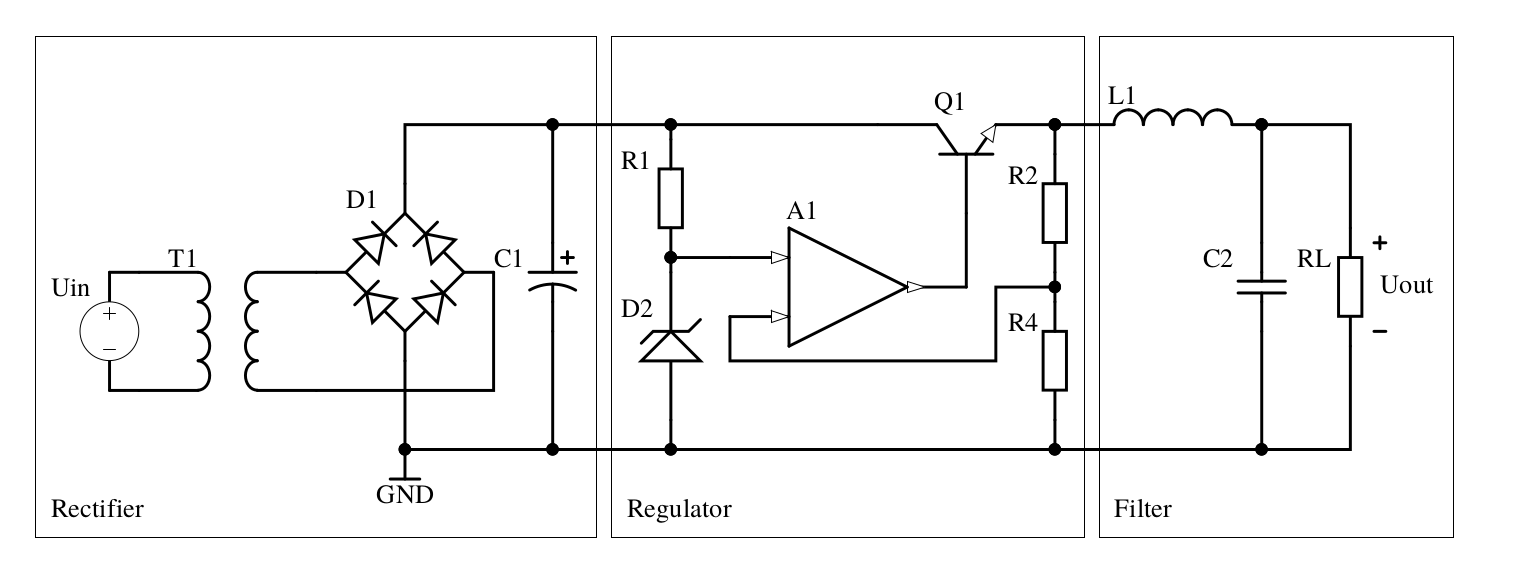
\includegraphics[width=\linewidth]{reg.png}
	\caption{DC voltage power supply device schematic}
	\label{fig:schematic}
\end{sidewaysfigure}

\clearpage

\subsection{Finding the proper choice of components}
\label{ele:task:1}
As it can be seen from the table \ref{tab:elems}, some components are not 
determined. 

\begin{table}[h!]
	\hyphenpenalty 10000
	\caption{Device element values}
	\label{tab:elems}
	\begin{tabularx}{\linewidth}{|X|X|X|X|} \hline
		ELEMENT & PARAMETER & VALUE & UNIT \\ \hline
		$T_1$ & transfer ratio ($n$) & $25$ &  dimensionless \\ \hline
		$D_1$ & $U_{pn}$ & $0.6$ & V \\ \hline 
		$R_2$ & Resistance & $1$ & M$\Omega$ \\ \hline
		$R_4$ & Resistance & $470$ & k$\Omega$ \\ \hline
		$R_L$ & Resistance & 10 & $\Omega$ \\ \hline
		$Q_1$ & $U_{pn}$ & $0.6$ & V \\ \hline
		$C_1$ & Capacitance & $10$ & mF \\ \hline
	\end{tabularx}
\end{table}
In this subtask you need to specify resistor $R_1$ and diode $D_2$. Based on 
the device operating values provided with table \ref{tab:spec} you have to 
determine specifications for the resistor $R_1$ and diode $D_2$. You have to 
find the components from the DigiKey Electronics product database. 

There are, however, constraints for your choice of components:
\begin{itemize}
	\item $R_1$ has footprint given with figure Fig. \ref{fig:footprint},
	\item $D_2$ is a through-hole component.
\end{itemize} 

Your choice is graded in several ways:
\begin{itemize}
	\item component price,
	\item correct component voltage, power and current ratings,
	\item correct component footprint.
\end{itemize}
As a result, you have to provide part number for resistor and part number for
diode, respectively.

\begin{figure}[h!]
	\centering
	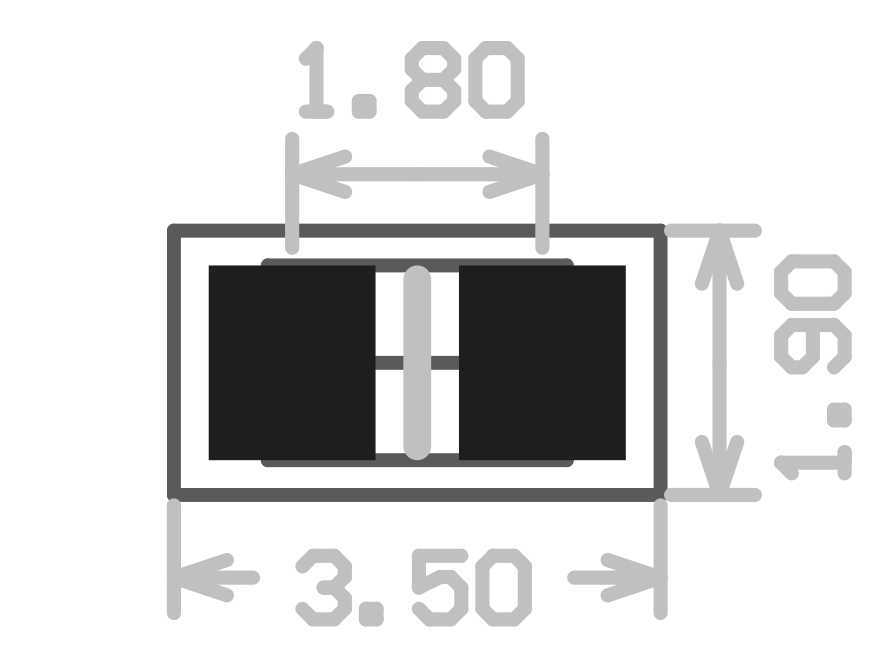
\includegraphics[width=0.5\linewidth]{footprint.png}
	\caption{Component footprint with dimension in millimeters}
	\label{fig:footprint}
\end{figure}

\newpage

\subsection{LC filter design}
\label{ele:task:2}
To achieve specified ripple rejection at required frequency, design a LC low 
pass filter which filters output of a regulator. As in previous task you have 
to provide DigiKey part numbers for LC filter. \textbf{Note:} The ripple 
rejection of the regulator part of the device is $58$ dB at $36$ kHz.

Again, there are constraints for your choice of components:
\begin{itemize}
	\item $L_1$ has no additional constraints 
	(think about already mentioned implicit constraints),
	\item $C_2$ has footprint given with Fig. \ref{fig:footprint},
	\item $Q$ factor has to be equal $\frac{\sqrt{2}}{2}$ for $R_L = 10$ 
	$\Omega$.  
\end{itemize}
$Q$ factor has to be as close to $\frac{\sqrt{2}}{2}$ as possible. 

Your choice is graded in the similar fashion as before:
\begin{itemize}
	\item price,
	\item correct inductance and capacitance,
	\item correct footprints, 
	\item correct current and voltage ratings.
\end{itemize}
As a result, you have to provide part number for inductor and 
part number for capacitor, respectively. 
\newpage
\subsection{Side task: Reliability of the system with redundant power supply} 
\label{ele:task:3}
To increase reliability of the power supply system two different linear 
regulators are linked in configuration which is given with the Fig. 
\ref{fig:psc}. This configuration is known as passive standby redundancy. 
Probability of a failure in one regulator is modeled with exponential 
probability density function. More precisely, probability density function for 
the first regulator is:  
\begin{equation}
f_1(t) = \lambda_1 e^{-\lambda_1 t}
\end{equation}
and for the second regulator:
\begin{equation}
f_2(t) = \lambda_2 e^{-\lambda_2 t}
\end{equation}

Your task is to determine probability density function $f_S(t)$ which gives the
probability of failure in system described with Fig. \ref{fig:psc}. As a result 
provide probability of a failure for $t = 10000$ $h$ with:
\begin{itemize}
	\item[] $\lambda_1 = 1 \cdot10^{-6}$ $h^{-1}$
	\item[] $\lambda_2 = 2 \cdot10^{-6}$ $h^{-1}$ 
\end{itemize} 

\textbf{Note}: mean time between failures is increased $T_{sf} = 
T_{1f} + T_{2f}$. 

\begin{figure}[h!]
	\centering
	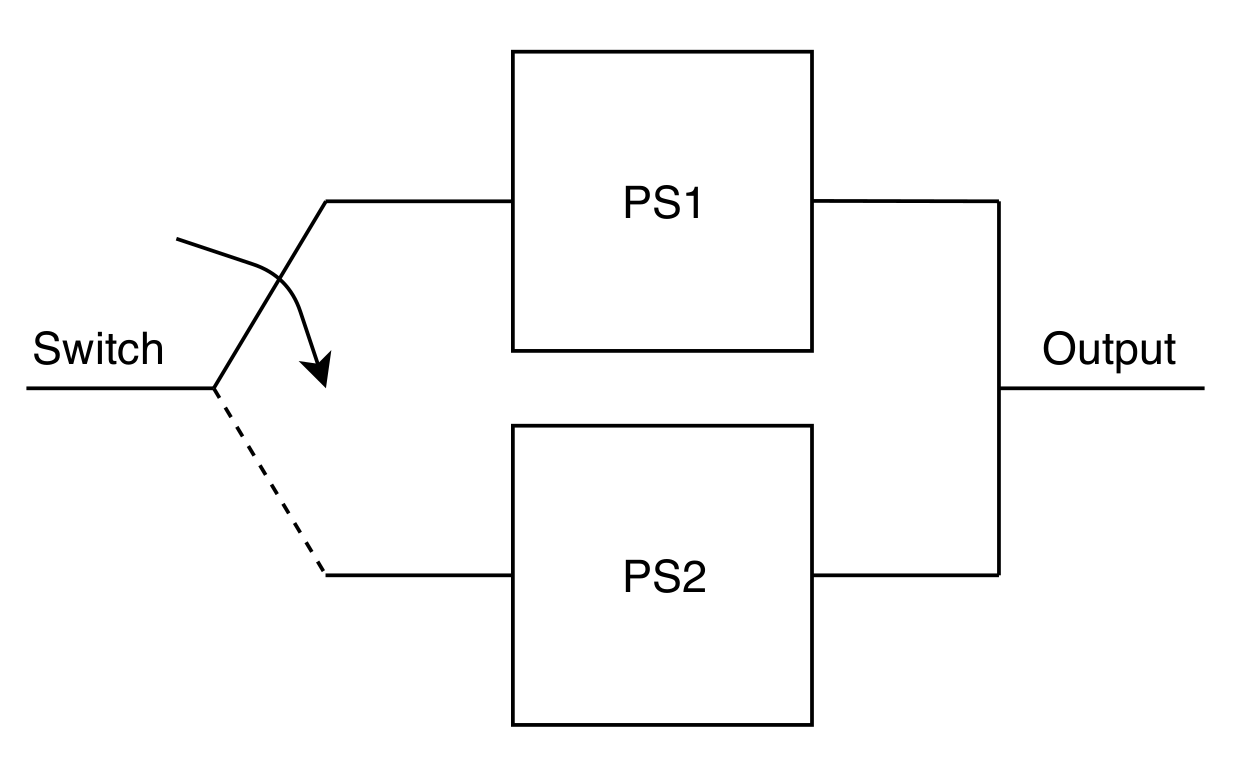
\includegraphics[width=\linewidth]{standby.png}
	\caption{Standby system configuration}
	\label{fig:psc}
\end{figure}

\newpage

\subsection{Solution format}
Solution for each task is a plain text document containing requested data. For
the tasks \ref{ele:task:1} and \ref{ele:task:2} text documents need to have 
two rows. One component part number in each row. Only one row is needed for the 
task \ref{ele:task:3} (requested probability). Name the files 
\texttt{task1.txt}, \texttt{task2.txt}, \texttt{task3.txt} and put them in 
the appropriate Google Drive folder.

Additionally, for the task \ref{ele:task:3} you have to provide paper 
documentation which has to contain derivation of $f_S(t)$.

\subsection{Grading scheme}
Tasks are graded in the following manner:
\begin{itemize}
	\item tasks \ref{ele:task:1} and \ref{ele:task:2} - up to \textbf{5 pts} 
	each (correct components in each task), 
	\item task \ref{ele:task:3} - up to \textbf{5 pts} - \textbf{2.5 pts} for 
	the correct probability and up to \textbf{2.5 pts} for correct 
	documentation.
\end{itemize}

\end{document}

